\section{Approach}

Based on weeks of literature reviewing and testing,
we have designed our overall approach to this task as followed:

\begin{enumerate}
    \item Energy-Based VAD

      Input audio signals are very likely to contain significantly large ratio of blank signals.
      VAD (Voice Activity Detector)
      is a preprocessing technique to filter out the blank period.
      The most common approach toward this goal is to use energy-based feature of signals.

      \item Cepstrum-Based Features

        Research showed that cepstrum-based features are more discrimitive in the task of speech and speaker recognition/verification.
        We decide to apply common cepstrum features extraction routine, such as MFCC (Mel-frequency Cepstrum Coefficients), LFCC,
        after the original signals are preprocessed by VAD.

       The basic procedure of MFCC is shown below, and the details about
       extracting MFCC is already been explained in the previous reports.
       The output of this step, is a sequence of fixed-dimension vectors, which will be used later in model training.

      \begin{figure}[H]
        \centering
        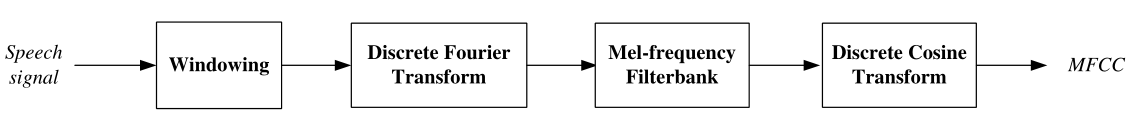
\includegraphics[width=\textwidth]{res/MFCC.png}
      \end{figure}

    \item GMM and UBM Model

      Since the feature vectors of a speaker tend to cluster into \textbf{several} groups
      in the feature space,
      the model of a specific speaker can be well described by using GMM (Gaussian Mixture Model).
      Moreover, for different speakers, the components of their individual GMMs
      will also have similar distributions, which discriminate different syllables.
      Therefore, an UBM (Universal Background Model) can be first trained for all speakers,
      and then we can get adapted GMMs which fit this task better.

      \begin{figure}[H]
        \centering
        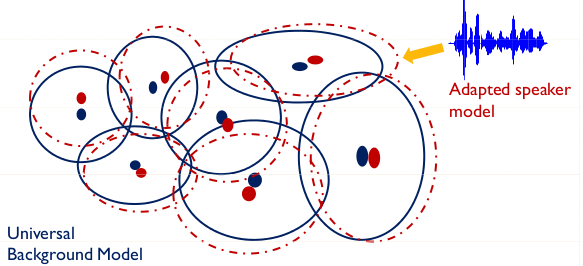
\includegraphics[width=0.7\textwidth]{res/ubm.png}
      \end{figure}

      \item JFA
        GMM-based model can describe the clusterred distribution, but it fails to account for
        different types of variability in each clusterred group.
        However, we only need inter-speaker variability to be modeled,
		but not channel or noise variability. Join Factor Analysis can convey
		such information.

  \end{enumerate}

